\chapter{Tor wizyjny z algorytmem Mean-shift}
\label{cha:torwizyjnyzalgorytmemmeanshift}

Przekształcono tor wizyjny zbudowany w rozdziale \ref{cha:torwizyjny} tak, by źródłem położenia obiektu był gotowy algorytm Mean-shift, który został opisany w podrozdziale \ref{sec:meanshift}. 
Rozpoczęto od zmiany otrzymanego modułu tak, by wielkości potrzebne do inicjalizacji algorytmu (rozmiar i początkowe położenie okna) były parametrami używanego modułu. Dzięki temu można je łatwo zmieniać.
%TODO niejasne. -zrobione. Mam nadzieję, że teraz lepiej.
Oprócz tego dodano sygnał wyjściowy informujący o wyznaczeniu nowego położenia środka obiektu. Potrzebny jest on do zgłoszenia przerwania w procesorze.

\paragraph*{}
Użyty algorytm Mean-shift wylicza wartości prawdopodobieństwa dla pikseli na podstawie histogramu ich otoczenia i histogramu początkowej ramki. Do modułu przekazywana jest jedna składowa przestrzeni barw.
%TODO to już wyjasniliśmy -zrobione. Trochę zmienione.
Jego działanie może być więc w dużej mierze zależne od wielkości podawanej na wejście.
%TODO powt. działanie -zrobione.
Postanowiono najpierw użyć wartości składowej Y z przestrzeni barw YUV.
Obliczana jest ona następująco:
\begin{equation}
\label{eq:grayscale}
Y=0.299 \cdot R+0.587 \cdot G+0.114 \cdot B
\end{equation}
Bierze się w ten sposób pod uwagę, że oko ludzkie jest najbardziej wyczulone na kolor zielony, a najmniej na kolor niebieski. 
Do wykonania powyższej konwersji zostały użyte 3 moduły mnożarki (DSP) w układzie FPGA.
Oprócz wartości piksela i sygnałów synchronizacyjnych na wejście podawany jest również sygnał ustawienia histogramu obiektu. 
Zapisywany jest wtedy histogram obiektu aktualnie znajdującego się w oknie. 
Sygnał ten został podłączony do przełącznika znajdującego się na karcie ZYBO. 
Wyjście modułu realizującego śledzenie zostało wyprowadzone do modułu, który na obrazie wyjściowym zaznacza aktualne okno.

\paragraph*{}
Najpierw sprawdzono działanie zaimplementowanego systemu podając na wejście HDMI obraz z komputera PC. 
Było nim czarne koło na białym tle. 
Przesuwano koło i sprawdzano, czy zaznaczone okno będzie się przesuwać razem z nim. 
Na podstawie wyników stwierdzono, że algorytm działa, lecz gubi obiekt, kiedy ten porusza się zbyt szybko, lub wykona jakiś gwałtowny ruch. 
Może to być bardzo problematyczne w trakcie śledzenia rzeczywistego obiektu. 
Dla obrazu z kamery nie będzie również tak dobrze rozróżniony obiekt od tła. 
Można się więc domyślać, że algorytm ten dużo gorzej będzie działać w rzeczywistym układzie.

\paragraph*{}
Następnie na wejście HDMI podano obraz z kamery używanej w projekcie.
Śledzono zielony prostokątny element.
Problemem okazał się wspomniany brak dobrego rozróżnienia obiektu od tła oraz wrażliwość zmian użytej składowej Y na zmiany oświetlenia.
W efekcie śledzony obiekt był bardzo często gubiony przez algorytm.
%TODO ostatnie zdanie niejasne. -zrobione.

\paragraph*{}
Aby zwiększyć efektywność testowanego algorytmu zmieniono sposób wyznaczania obrazu w skali szarości. 
Zamiast obliczania składowej Y przestrzeni YUV do modułu śledzącego podano składową H przestrzeni barw HSV. 
Odpowiada ona za kolor obiektu, więc powinna dać lepsze wyniki gdy obiekt ma inny kolor niż otoczenie \cite{Kryjak}.
\begin{equation}
V=max(R,G,B)
\end{equation}
\begin{equation}
S=
	\begin{cases}
	\frac{V-min(R,G,B)}{V} &\text{jeśli } V \neq 0\\
	0 &\text{jeśli } V=0
	\end{cases}
\end{equation}
\begin{equation}
H=
	\begin{cases}
	0 &\text{jeśli } V-min(R,G,B)=0\\
	\frac{60(G-B)}{V-min(R,G,B)} &\text{jeśli } V=R\\
	\frac{60(B-R)}{V-min(R,G,B)}+120 &\text{jeśli } V=G\\
	\frac{60(R-G)}{V-min(R,G,B)}+240 &\text{jeśli } V=R
	\end{cases}
\end{equation}
\begin{equation}
H \leftarrow
	\begin{cases}
	\frac{H+360}{360} &\text{jeśli } H<0\\
	\frac{H}{360} &\text{jeśli } H \geqslant 0
	\end{cases}
\end{equation}
Zmiana ta podyktowana jest faktem, że śledzony obiekt jest koloru zielonego, a w otoczeniu występuje niewiele elementów tego koloru. W wyniku opisanej zmiany algorytm Mean-shift zaczął dużo lepiej śledzić testowy obiekt. Gubiony był on w tylko wyniku zbyt nagłego ruchu obiektu lub gdy zmieniał się kolor tła.

%TODO OK, ale to w takim razie tam proszę podać, że moduł przujmuje jedną wybraną składową i przetestowano Y i H.
%MK: "Do modułu przekazywana jest jedna składowa przestrzeni barw." Zmieniłem na coś takiego.
\newpage
Na rysunku \ref{fig:meanshift_servo} przedstawiono zdjęcie z testów działania kompletnego systemu z algorytmem Mean-shift. 

\begin{figure}[h]
	\centering
	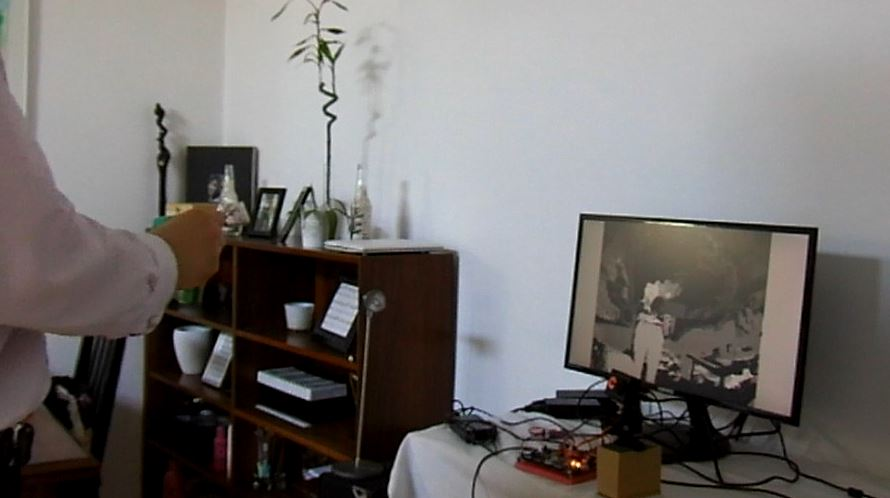
\includegraphics[width=4in]{meanshift_servo.jpg}
	\caption{Zdjęcie z testów działania systemu z algorytmem Mean-shift.}
	\label{fig:meanshift_servo}
\end{figure}

Układ był poprawnie pozycjonowany tak, by śledzony obiekt znajdował się w środku kadru. Negatywnie na działanie układu wpływały szybkie przemieszczenia obiektu (był on wtedy gubiony). Zaletą tego rozwiązania były małe wahania współrzędnych wyznaczonego środka, gdy obiekt nie poruszał się. W efekcie system nie wykonywał drgań wokół środka obiektu.